% !TeX program = xelatex
\documentclass[aspectratio=169]{beamer}
\usepackage{booktabs}
\usetheme{metropolis}           % Use metropolis theme
\title[Practical Encoded Dynamic Bulk]{Lecture V: The Item RAM Strikes Back!}
\subtitle{Towards a practical dynamic bulk storage system for use in the real world}
\date{}
\author{\textbf{Instructor:} Andrews54757}
\institute{
    CSE269: Introduction to Encoded Storage\\
    S$\infty$ntech Annals
}
\logo{
\includegraphics[height=0.7cm]{logo3.png}}
\begin{document}
\maketitle

\begin{frame}
\frametitle{Overview}
\tableofcontents
\end{frame}

\AtBeginSection{}
\setbeamertemplate{caption}{\raggedright\insertcaption\par}

\section{1. What is dynamic bulk?}

\begin{frame}
	\frametitle{1. What is dynamic bulk?}

    \begin{itemize}
		\item \textbf{Static bulk} has a fixed capacity for each item type
        \item \textbf{Dynamic bulk} automatically expands and shrinks capacity for items
	\end{itemize}

	\begin{figure}
        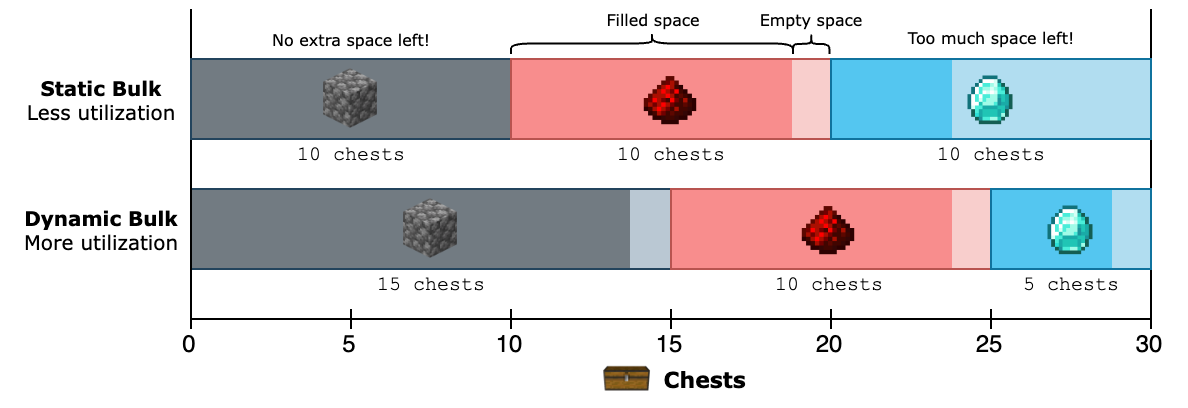
\includegraphics[width=0.95\textwidth]{dynstatic.png}
	\end{figure}
\end{frame}

\begin{frame}
	\frametitle{1. What is dynamic bulk? Contd.}

    \begin{itemize}
		\item Divide your storage into \textbf{slices} of fixed size
        \item Each slice can store a fixed number of items
        \item The size of your slice determines the minimum non-zero amount of storage space you can allocate to an item type
	\end{itemize}

    \begin{figure}
        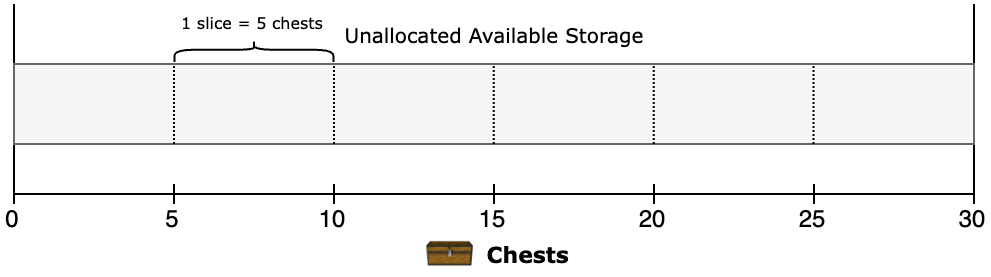
\includegraphics[width=0.95\textwidth]{logic0.png}
	\end{figure}


\end{frame}


\begin{frame}
	\frametitle{1. What is dynamic bulk? Contd.}

    \begin{itemize}
		\item Let's store 8 chests of redstone
        \begin{itemize}
		\item Do we have a slice assigned to redstone? \textbf{No!}
        \item Allocate an available slice to redstone
        \item Now we have space to start storing redstone!
        \end{itemize}
	\end{itemize}

    \begin{figure}
        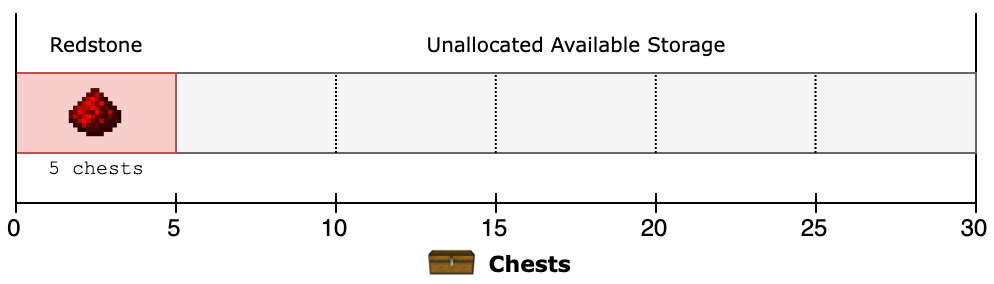
\includegraphics[width=0.95\textwidth]{logic1.png}
	\end{figure}
\end{frame}

\begin{frame}
	\frametitle{1. What is dynamic bulk? Contd.}

    \begin{itemize}
		\item Let's store 8 chests of redstone
        \begin{itemize}
        \item Fully filled one chest with 5 chests of redstone
		\item But we have more 3 more chests of redstone to store!
        \end{itemize}
	\end{itemize}

    \begin{figure}
        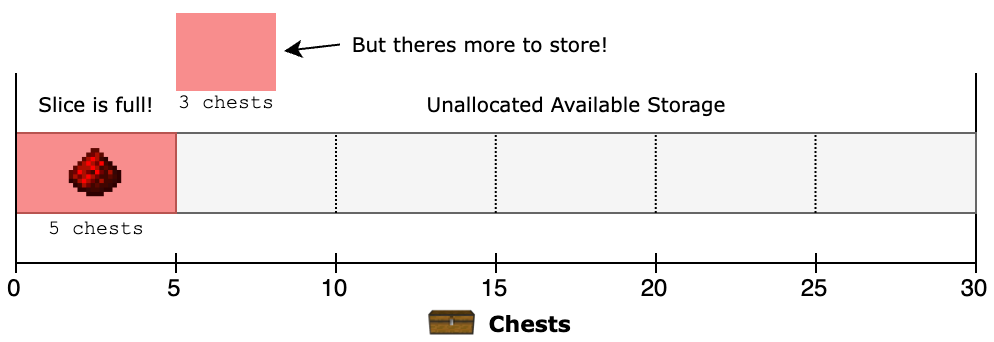
\includegraphics[width=0.95\textwidth]{logic2.png}
	\end{figure}
\end{frame}


\begin{frame}
	\frametitle{1. What is dynamic bulk? Contd.}

    \begin{itemize}
		\item Let's store 8 chests of redstone
        \begin{itemize}
        \item One slice is \textbf{fully} filled with redstone (5 chests)
        \item Another slice is \textbf{partially} filled with redstone (3 chests / 5 chests)
        \end{itemize}
	\end{itemize}

    \begin{figure}
        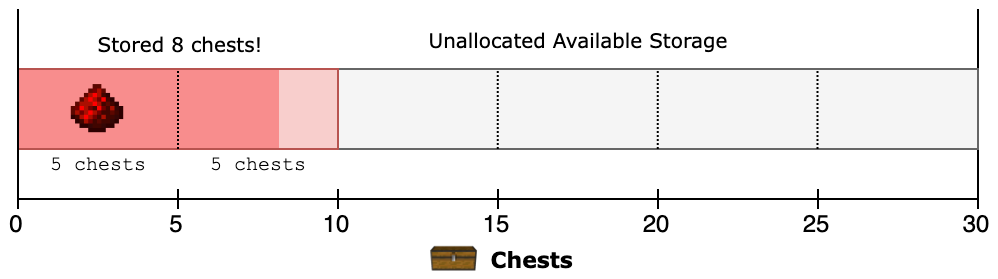
\includegraphics[width=0.95\textwidth]{logic3.png}
	\end{figure}
\end{frame}

\begin{frame}
	\frametitle{1. What is dynamic bulk? Contd.}

    \begin{itemize}
		\item Retrieve 1 chest of redstone
        \begin{itemize}
        \item Pull from the partially filled slice first!
        \item Minimize internal fragmentation
        \end{itemize}
	\end{itemize}

    \begin{figure}
        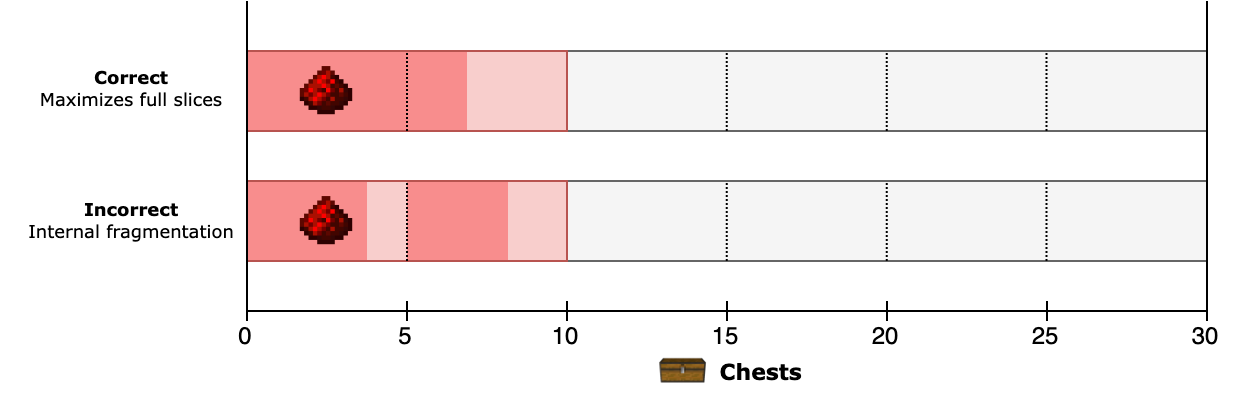
\includegraphics[width=0.95\textwidth]{logic4.png}
	\end{figure}
\end{frame}


\section{2. Fast and compact data storage is hard}

\begin{frame}
	\frametitle{2. Fast and compact data storage is hard}

    \begin{itemize}
		\item We need to keep track of what slices are assigned to each item type
        \item Must store that information in a way that is quickly accessible
        \item Storage must be dense so that it is compact
	\end{itemize}

    \begin{figure}
        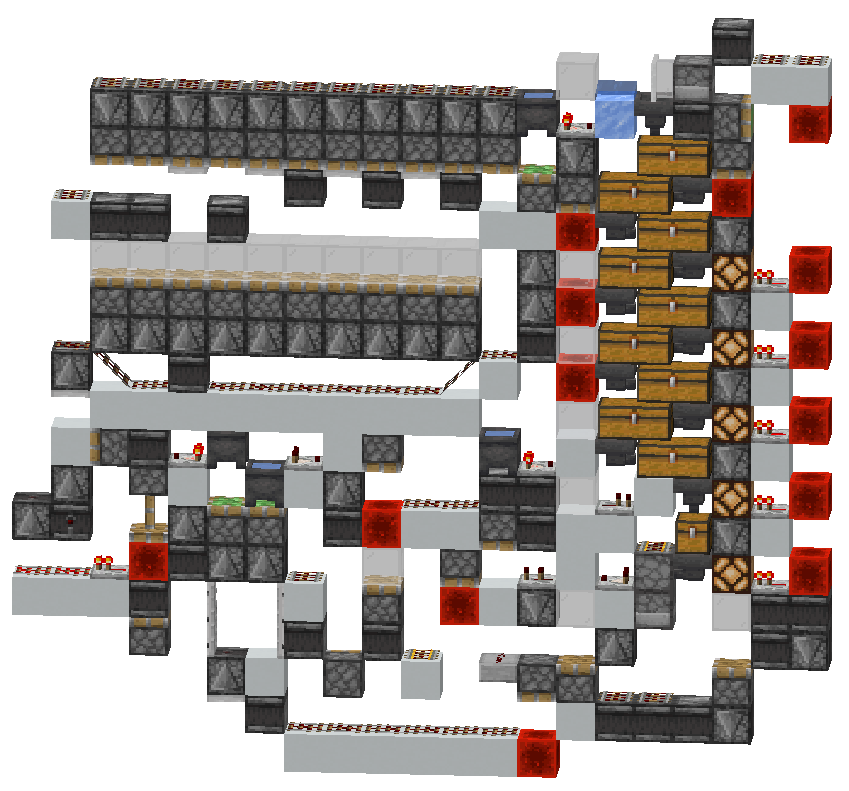
\includegraphics[width=0.25\textwidth]{pallaslice2.png}
        \hfill
        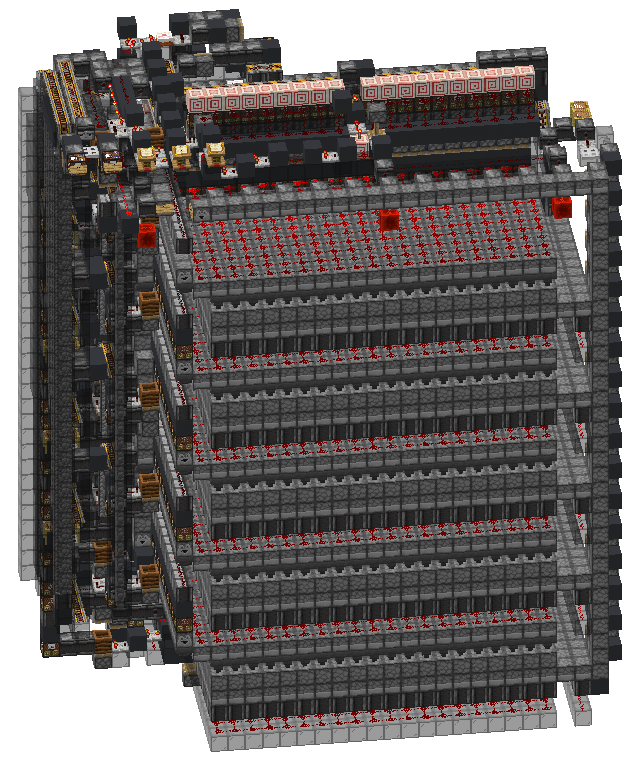
\includegraphics[width=0.18\textwidth]{bigram.png}
        \hfill
        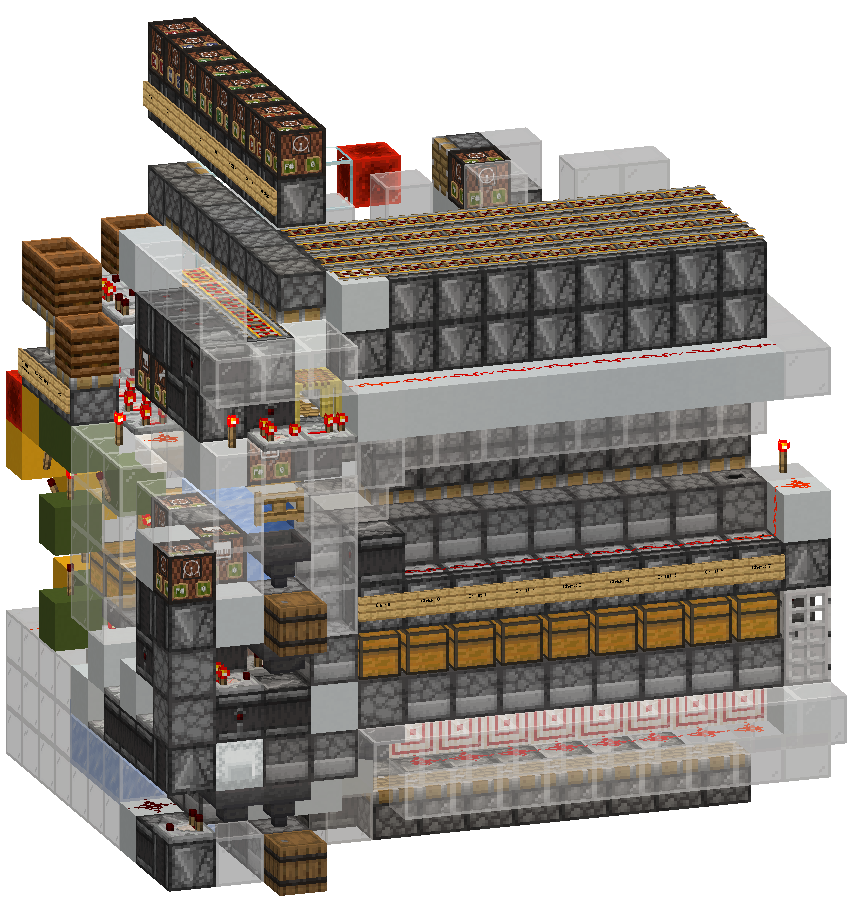
\includegraphics[width=0.22\textwidth]{diskdrive.png}
        \hfill

        \caption{\textbf{From left to right:} PallaPalla's Dynamic Slice, 1000 Item RAM, Obi's Disk Drive}
	\end{figure}
\end{frame}

\subsection{2.1 Internal logic has problems}

\begin{frame}
	\frametitle{2.1 Internal logic has problems}

    \begin{itemize}
		\item PallaPalla, original inventor of dynamic bulk, uses a binary re-mappable decoder to store assigned item code within each slice.
		\item Almost every piston in each slice's decoder is fired to write/test item codes. Laggy and higher chance of data corruption.
		\item Allocation logic is internal to the slice, so each slice is large and complex.
	\end{itemize}

    \begin{figure}
        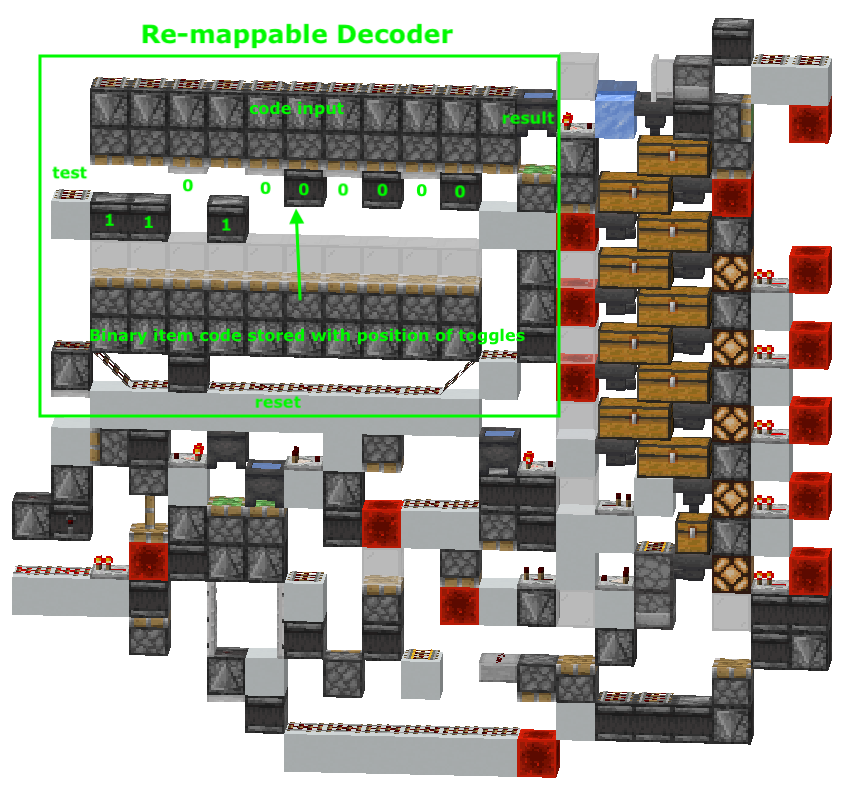
\includegraphics[width=0.25\textwidth]{pallaslice2lbl.png}
        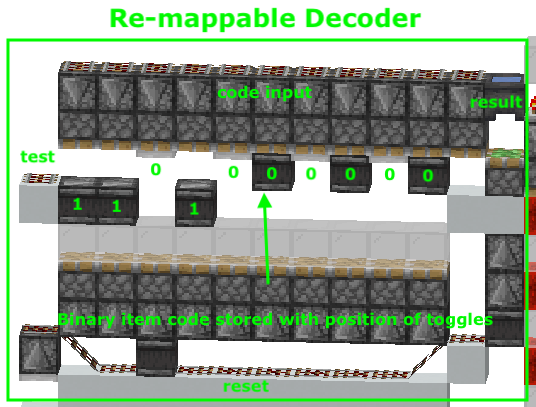
\includegraphics[width=0.33\textwidth]{pallaslice2lblzoom.png}
    \end{figure}

\end{frame}

\begin{frame}
	\frametitle{2.1 Internal logic has problems. Contd.}

    \begin{itemize}
		\item What if we externalized the slice allocation logic?
        \begin{itemize}
        \item Each slice is now just a simple static encoded bulk unit
        \item Store information about slice allocation in a separate memory unit
        \item Externalized logic is simpler and more compact
        \end{itemize}
	\end{itemize}
    \begin{figure}
        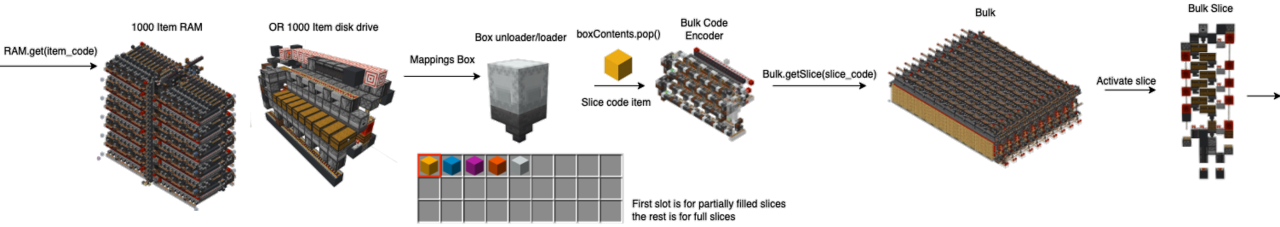
\includegraphics[width=0.98\textwidth]{dynamicbulk2.png}
        \caption{\textbf{Figure 12:} Diagram of dynamic bulk with externalized logic}
	
    \end{figure}

\end{frame}


\begin{frame}
	\frametitle{2.1 Internal logic has problems. Contd.}

    \begin{itemize}
		\item How is slice allocation information stored externally?
        \begin{itemize}
        \item Represent slices with an encodeable item called the \textbf{slice code item}. One slice code item corresponds to one slice.
        \item Maintain a list of slice code items in box dedicated to one item type
        \item Store the list of slice code items in an external item memory unit in the address corresponding to the item type
        \end{itemize}
	\end{itemize}
    \begin{figure}
        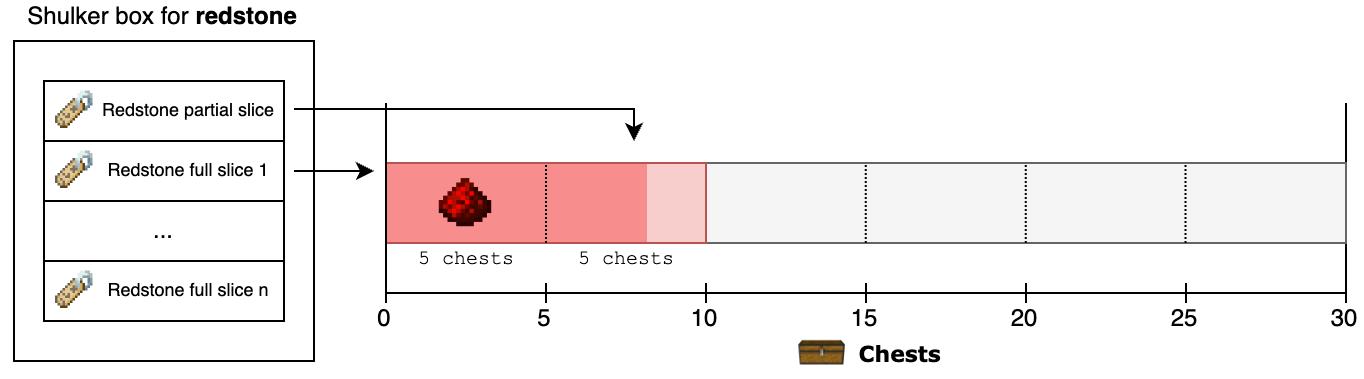
\includegraphics[width=0.8\textwidth]{externallayout.png}
        \caption{\textbf{Figure 12:} Externalized dynamic bulk data layout}
	
    \end{figure}

\end{frame}


\subsection{2.2 Item RAMs are fast but large}


\begin{frame}
	\frametitle{2.2 Item RAMs are fast but large}

    \begin{itemize}
		\item An item RAM is a memory unit that stores items in an addressible way
        \item Each item type is assigned a unique address
        \item The item RAM can be read from and written quickly in constant time (O(1))
	\end{itemize}
    \begin{figure}
        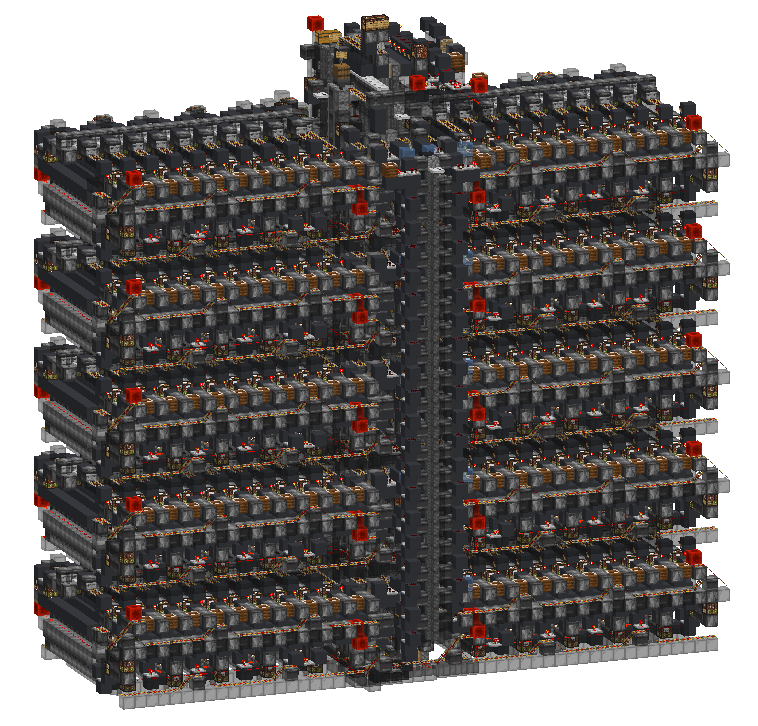
\includegraphics[width=0.3\textwidth]{bigbigram.png}
        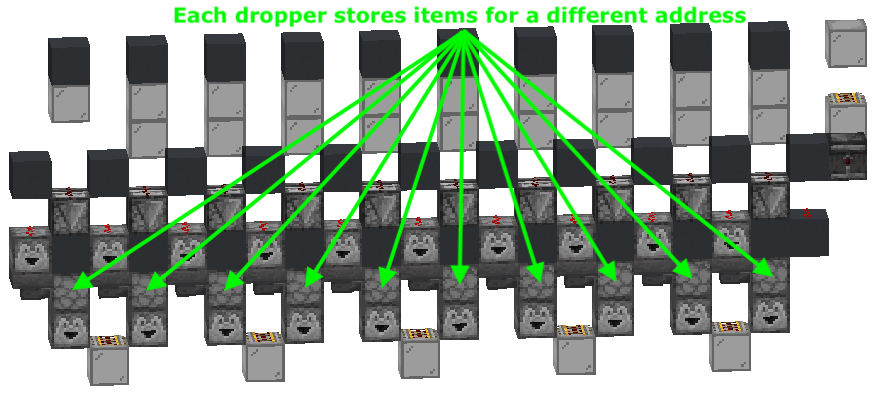
\includegraphics[width=0.6\textwidth]{bigbigramslice.png}
        \caption{\textbf{Figure 13-14:} 1000 address item RAM and its slice. 46gt call latency.}
	
    \end{figure}
\end{frame}

\begin{frame}
	\frametitle{2.2 Item RAMs are fast but large. Contd.}

    \begin{itemize}
		\item Unfortunately, item RAMs are very big.
		\item Latest advancements have doubled the density, but still too big.
		\item 17 x 41 x 33 blocks for 1000 addresses
	\end{itemize}
    \begin{figure}
        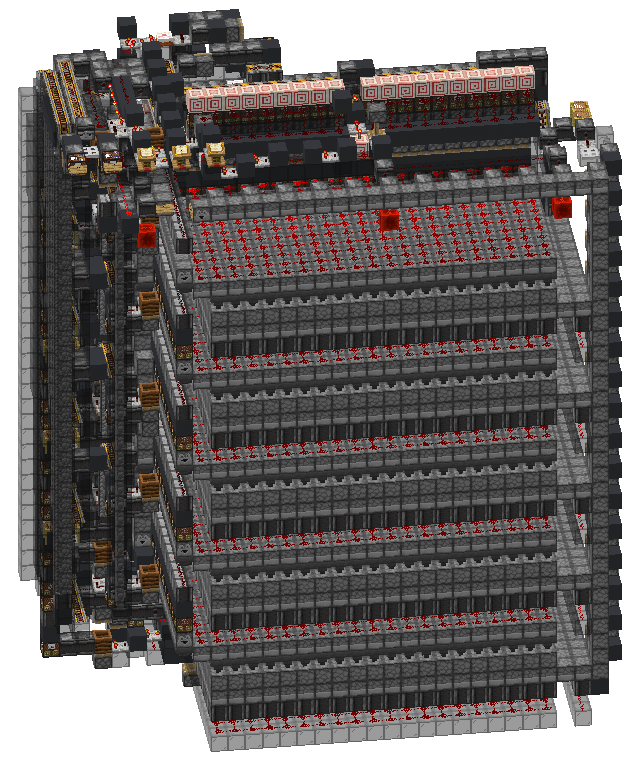
\includegraphics[width=0.2\textwidth]{bigram.png}
        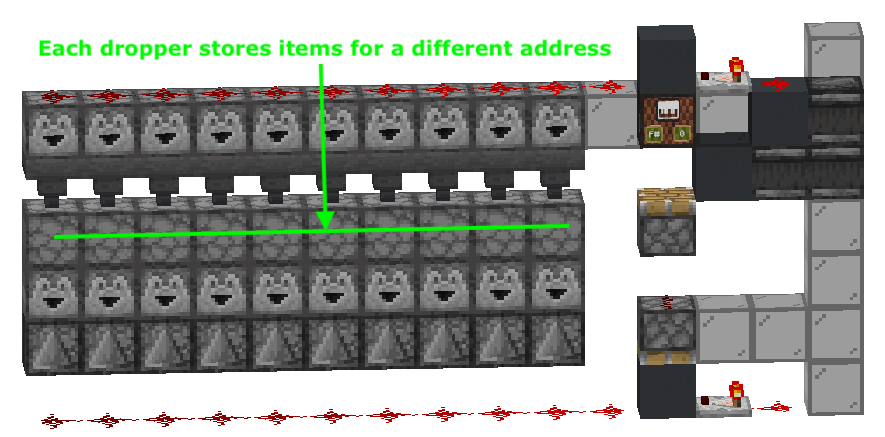
\includegraphics[width=0.55\textwidth]{bigramslice.png}
        \caption{\textbf{Figure 15-16:} Improved 1000 address item RAM and its slice. 46gt call latency.}
	
    \end{figure}
\end{frame}

\subsection{2.3 Disk drives are small but slow}

\begin{frame}
	\frametitle{2.3 Disk drives are small but slow}

    \begin{itemize}
		\item What if, we stored multiple boxes from different addresses in a single block?
		\item Store up to 54 boxes in a double chest
		\item Cycle through the boxes to find the correct one
	\end{itemize}
    \begin{figure}
        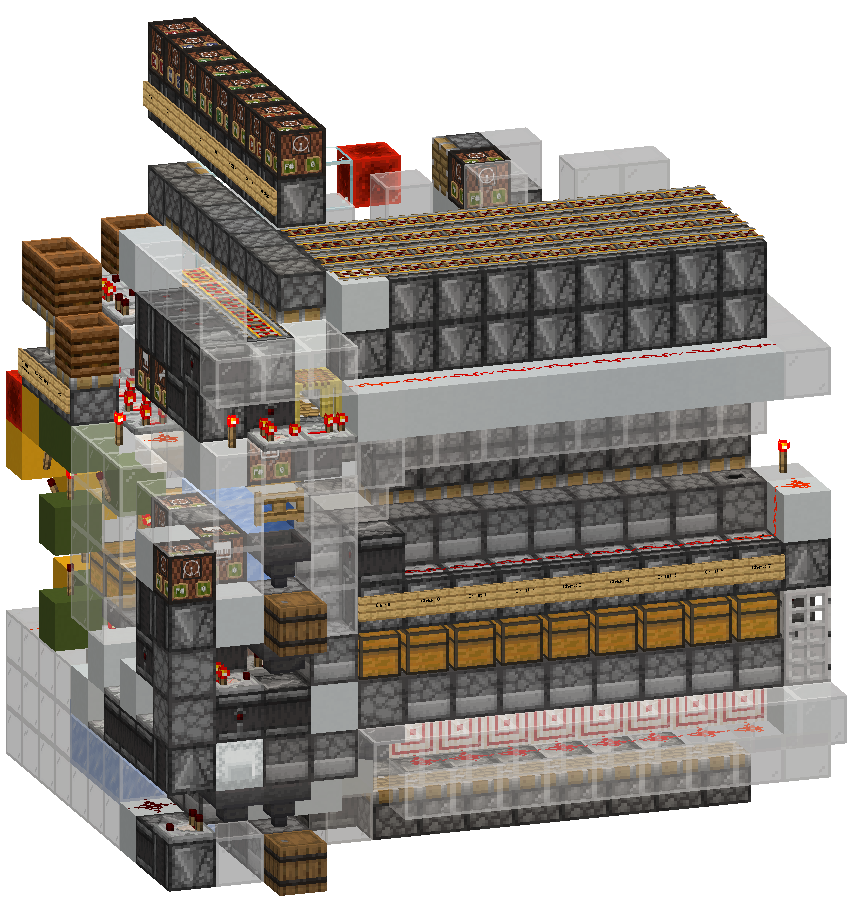
\includegraphics[width=0.25\textwidth]{diskdrive.png}
        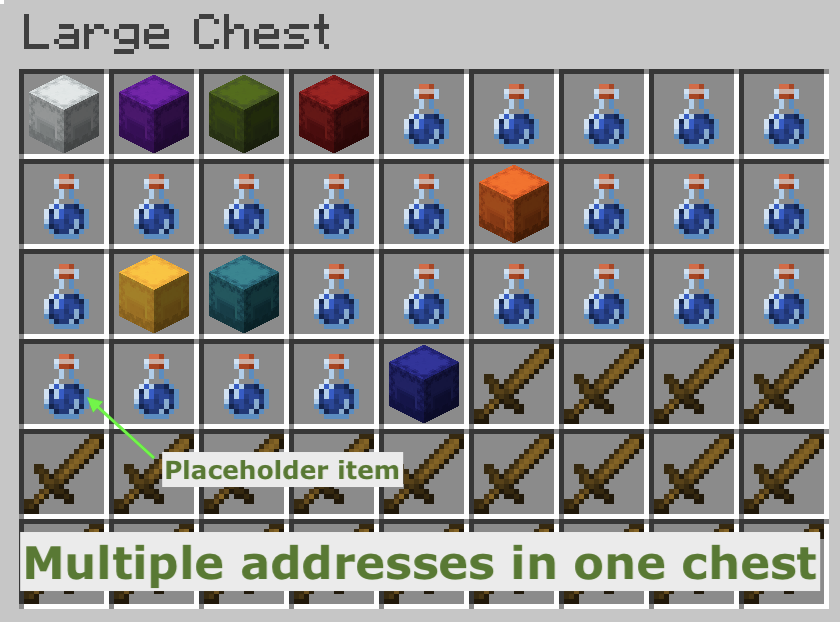
\includegraphics[width=0.35\textwidth]{diskcontent.png}
        \caption{\textbf{Figure 17-18:} Obi's Disk Drive, 256 addresses.}
    \end{figure}
\end{frame}



\begin{frame}
	\frametitle{2.3 Disk drives are small but slow. Contd.}

    \begin{itemize}
		\item Cycling through slots is slow, 8gt per slot.
		\item Box at the 32nd slot takes a minimum 248gt to access, which is 12.4 seconds.
		\item Need something faster!
	\end{itemize}
    \begin{figure}
        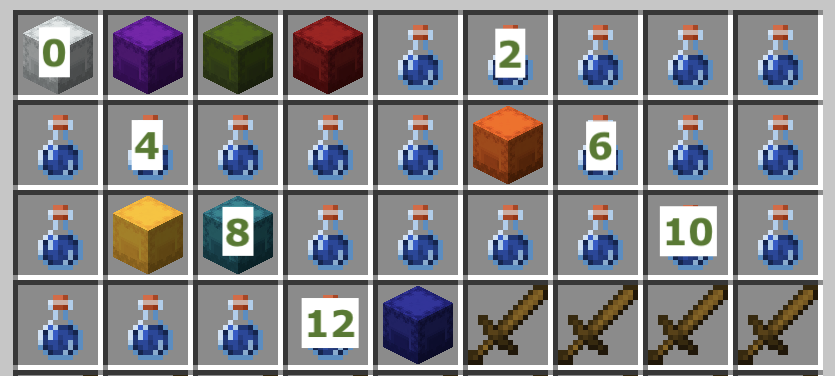
\includegraphics[width=0.5\textwidth]{diskcontent2.png}
        \caption{\textbf{Figure 19:} Minimum time in seconds to reach slot in a disk drive}
    \end{figure}
\end{frame}


\section{3. Solution: Linked-list based dynamic bulk}

% To recap, item RAMs are too big, and Disk drives are small but slow. The ideal solution would be a device that combines the best of both worlds to have both fast retrieval time and a compact size. Such a device would revolutionize the way we build dynamic bulk storage systems, making them more efficient and easier to implement.

% How can we achieve this? To answer that question, we need to seek inspiration from the world of computer science to develop a new  approach to dynamic bulk storage systems.

\subsection{3.1 Analysis of the problem}

\begin{frame}
	\frametitle{3.1 Analysis of the problem}

    \begin{columns}
        \column{0.55\linewidth}
    \begin{itemize}
		\item Item RAMs are fast but too big
        \item Disk drives are compact but too slow
        \item We need something that is both fast and compact
        \item \textbf{Towards a solution:} Get inspiration from computer science
	\end{itemize}

    \column{0.4\linewidth}
        
        \begin{figure}
        		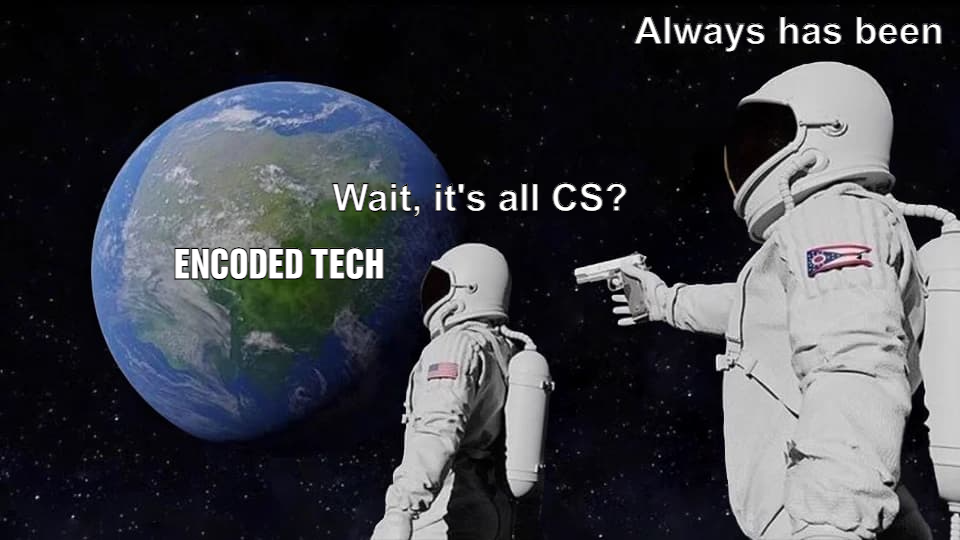
\includegraphics[width=1\textwidth]{meme.png}
        \end{figure}
    \end{columns}
\end{frame}

% Lets make some observations. Recall that it is important to retrieve a specific box out of a thousand quickly because any delay in this step will increase the wait time for the requested items to arrive. But does the system need to know all the slices allocated to an item type at once?

% No, it doesn't. The system only needs to know the partial slice first, as it is the slice that will be emptied or filled first. Filling and emptying takes a while anyway, so the system can take its time to find the other slices allocated to the item type. We only need to be quick with queries for the partial slice and the rest can be done in the background.

\begin{frame}
	\frametitle{3.1 Analysis of the problem. Contd.}

    \begin{itemize}
		\item Observations:
        \begin{itemize}
            \item System only needs to know the partial slice first
            \item Filling and emptying takes a while
            \item Rest of the slices can be slowly found in the background
        \end{itemize}
        \item \textbf{Idea:} Seperate the storage of partial slice information from the rest
	\end{itemize}

    \begin{figure}
        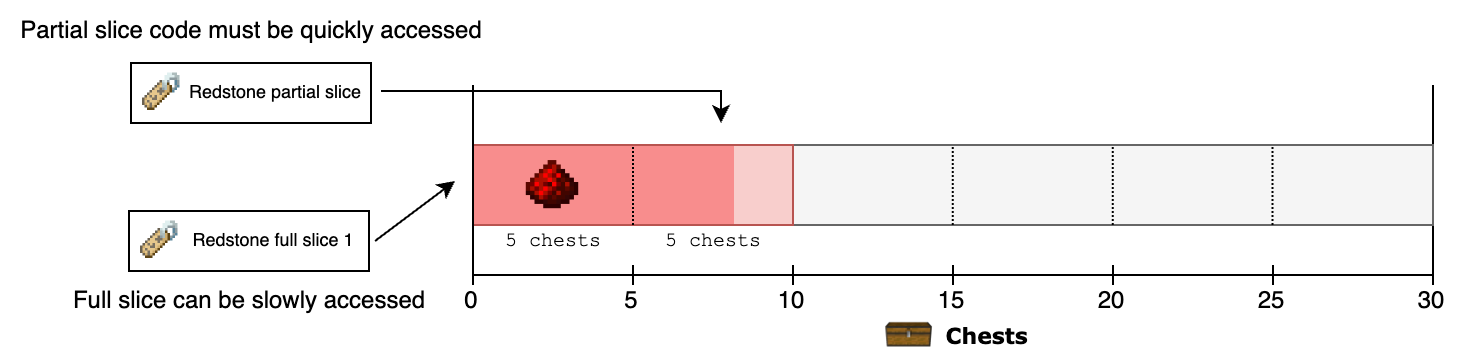
\includegraphics[width=1\textwidth]{fastslow.png}
    \end{figure}
\end{frame}

\begin{frame}
	\frametitle{3.1 Analysis of the problem. Contd.}

    \begin{itemize}
		\item \textbf{Lazy loading:} Defer loading an object until it is needed
        \item Store only the partial slice codes in a separate storage device with rapid access
        \item Slowly access information about other slices in the background as needed
	\end{itemize}
    \begin{figure}
        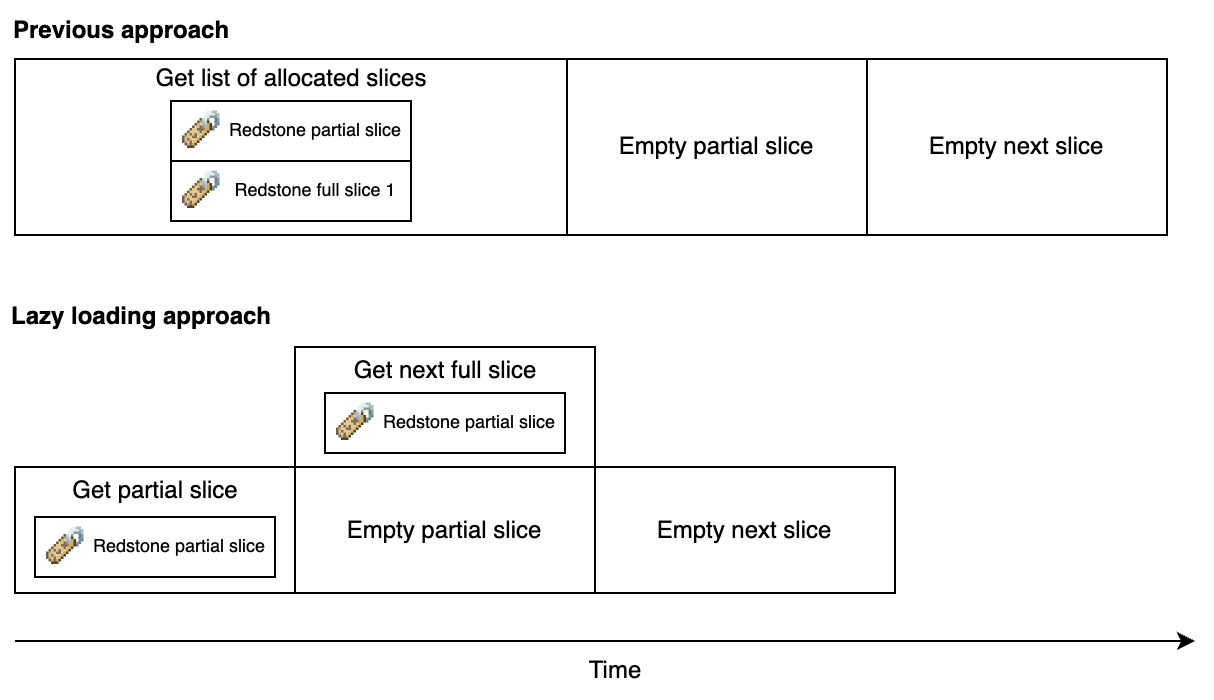
\includegraphics[width=0.65\textwidth]{lazy.png}
    \end{figure}
\end{frame}

\begin{frame}
	\frametitle{3.1 Analysis of the problem. Contd.}

    \begin{itemize}
		\item \textbf{Linked list:} Sequence of elements where each element points to the next
        \item Efficient insertion and deletion at the start of the list
        \item Slower access time to elements in the middle and end
	\end{itemize}
    \begin{figure}
        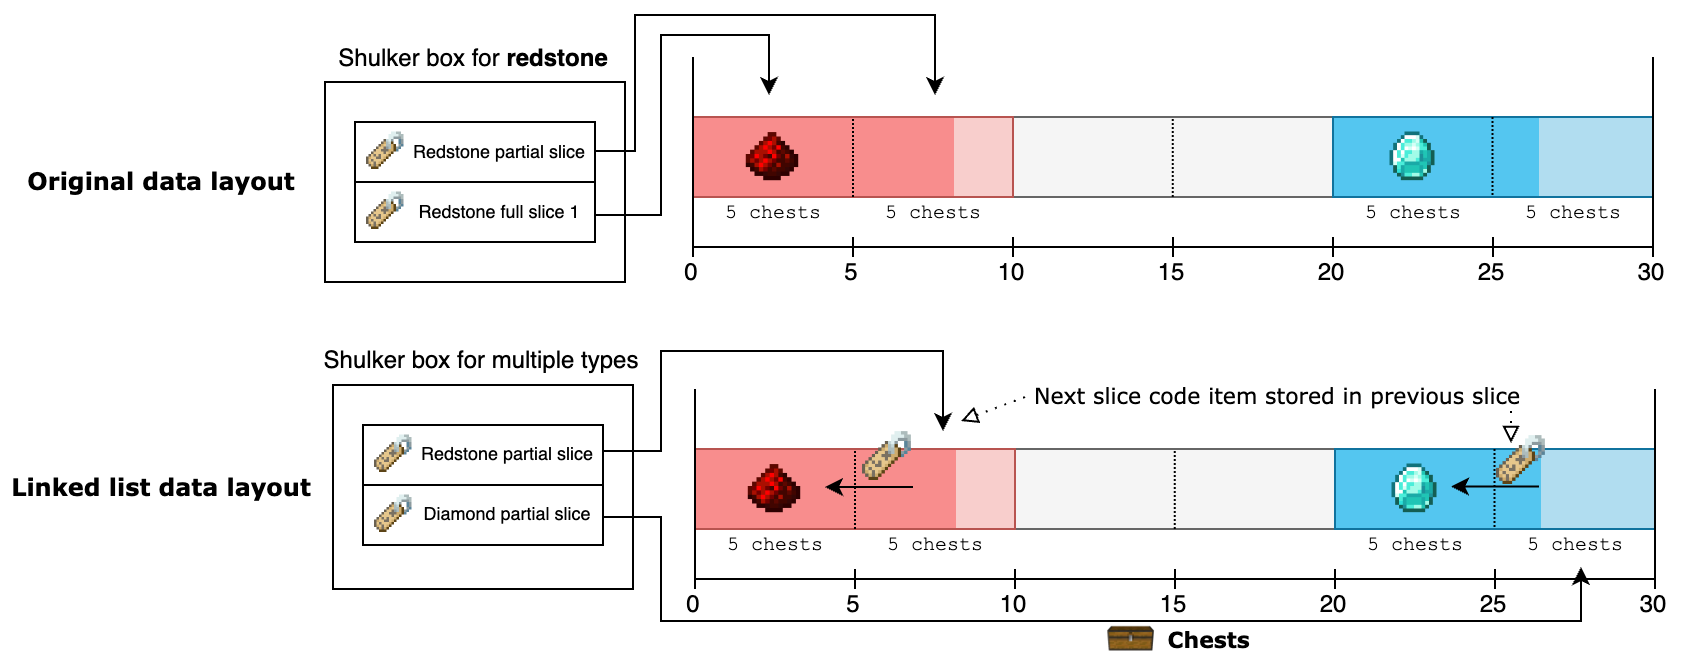
\includegraphics[width=0.95\textwidth]{layout2.png}
    \end{figure}
\end{frame}


\subsection{3.2 Implementation}

\begin{frame}
	\frametitle{3.2 Implementation}

    \begin{itemize}
		\item If instead of storing boxes, we store a single non-box slice code item per address
		\item Can pack multiple addresses in a single shulker box for higher density
	\end{itemize}
    \begin{figure}
        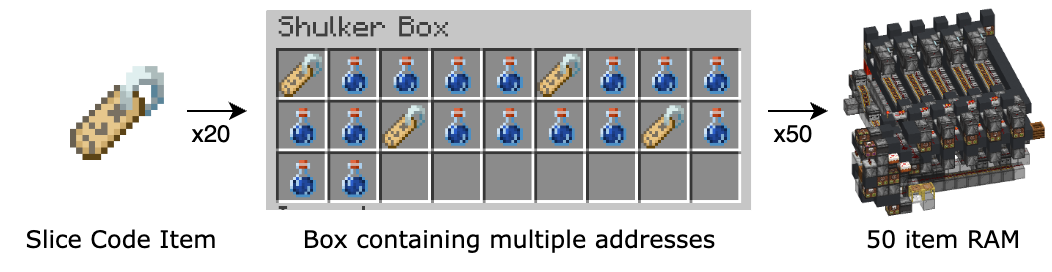
\includegraphics[width=0.8\textwidth]{nonboxlayout.png}
        \caption{\textbf{Figure 24:} Non-box item RAM storage scheme}
    \end{figure}
\end{frame}


\begin{frame}
	\frametitle{3.2 Implementation. Contd.}

    \begin{itemize}
		\item Using hoppercarts, can pull items from shulker boxes every game tick
        \item 8x faster cycling than traditional disk drives. Item at the 20th slot takes only 1 second
		\item We can quickly bring boxes to the ultrafast slot cycler using instant droppers
	\end{itemize}
    \begin{figure}
        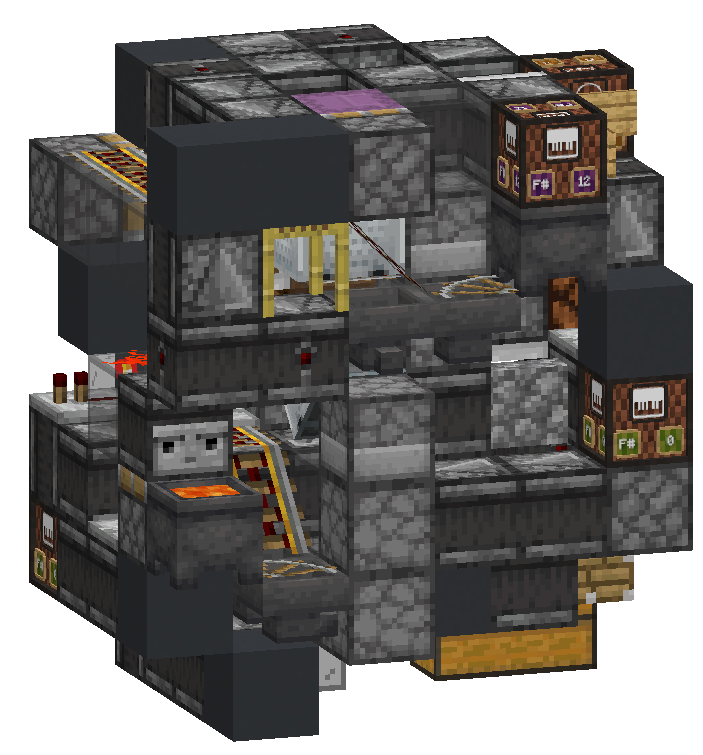
\includegraphics[width=0.15\textwidth]{slotiter.png}
        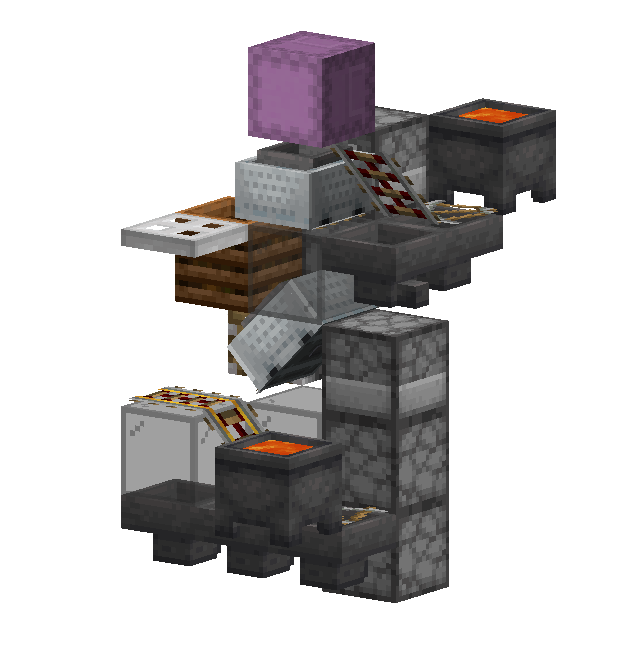
\includegraphics[width=0.15\textwidth]{slotintern.png}
        \caption{\textbf{Figure 25-26:} 1 slot/gt slot cycler with internal layout}
    \end{figure}
\end{frame}


\begin{frame}
	\frametitle{3.2 Implementation. Contd.}

    \begin{itemize}
		\item Combine slot cycler with 50 item RAM (21gt call latency)
		\item Can access 1000 addresses within 55gt
		\item Result: Both fast and compact!
	\end{itemize}
    \begin{figure}
        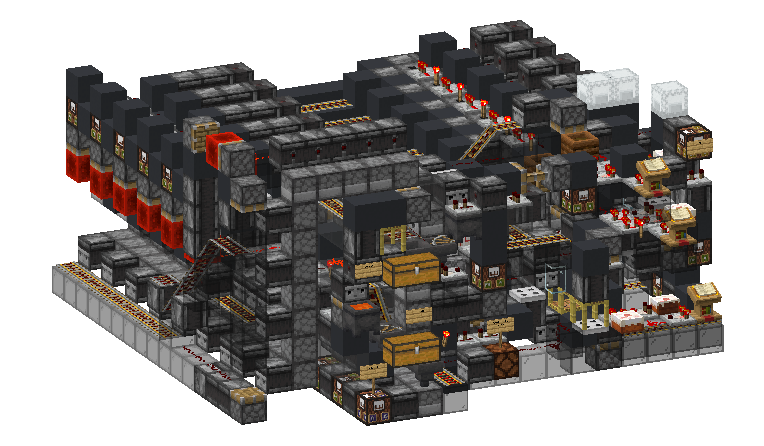
\includegraphics[width=0.4\textwidth]{nonbox.png}
        \caption{\textbf{Figure 27:} 1000 address non box item RAM}
    \end{figure}
\end{frame}


\begin{frame}
	\frametitle{3.2 Implementation. Contd.}

    \begin{itemize}
        \item Maintaining the linked list for \textbf{insertion} is simple.
        \begin{enumerate}
            \item Obtain a slice code item at a slot corresponding to the item code using the 1000 non-box-item RAM.
            \item Insert boxes into the corresponding slice.
            \item If slice is full, pull a new slice code item from storage to allocate a new empty slice
            \item Put the now-full slice code item into the newly allocated slice and put the rest of the boxes into the newly allocated slice. Repeat 3-4 as needed.
            \item Store the remaining slice code item into the 1000 non-box-item RAM at the slot corresponding to the item code to finish insertion.
        \end{enumerate}
    \end{itemize}
\end{frame}

\begin{frame}
	\frametitle{3.2 Implementation. Contd.}

    \begin{itemize}
        \item Maintaining the linked list for \textbf{retreival} is also simple.
        \begin{enumerate}
            \item Obtain a slice code item at a slot corresponding to the item code using the 1000 non-box-item RAM.
            \item Retrieve boxes from the corresponding slice. Test items if they are boxes, if one is not a box then hold it for later, it is the slice code item for the next slice.
            \item If slice is empty and you have found a code item for the next slice, then switch to the next slice. Put the now empty slice code item back into storage.
            \item Keep retreiving boxes, repeat 2-3 as needed.
            \item If you have found the slice code item for the next slice, put it back into the slice.
            \item Store the remaining slice code item into the 1000 non-box-item RAM at the slot corresponding to the item code to finish insertion.
        \end{enumerate}
    \end{itemize}
\end{frame}

\section{4. Conclusion and future steps}

\begin{frame}
    \frametitle{4. Conclusion and future steps}

    \begin{itemize}
        \item Linked-list based dynamic bulk has the potential to be both fast and compact
        \item Future work: Implement the linked-list based dynamic bulk and test its performance
        \item Further optimizations: Reduce the latency of the non-box item RAM
        \item \textbf{This is an assignment for you!} Unfortunately I have no time to implement this myself. Good luck!
        \begin{itemize}
            \item I have posted the schematic of the 1000 address non-box item RAM in the description to help you get started
        \end{itemize}
    \end{itemize}
\end{frame}



% \subsection{1.1 Basic Optimizations}

% \begin{frame}
% 	\frametitle{1.1 Basic Loader Optimizations}
    

% 	\begin{figure}
%         \includegraphics[width=0.3\textwidth]{oldloader.png}
% 		\includegraphics[width=0.35\textwidth]{newloader.png}
% 		\caption{Old 4x loader (left) vs new 8x loader (right)}
% 	\end{figure}


%     \begin{itemize}
% 		\item Twice as fast so half the latency
% 		\item Less hoppers per hopperspeed (3 vs 1.38)
% 		\item Less loaders = simpler logic
% 	\end{itemize}
	
% \end{frame}

% \begin{frame}
% 	\frametitle{1.1 Basic Loader Optimizations Contd.}
%     \begin{columns}
%         \column{0.4\linewidth}

% 	\begin{figure}
% 		\includegraphics[width=1\textwidth]{toploaderview.png}
% 		\caption{Loader layout}
% 	\end{figure}

%     \column{0.6\linewidth}
%     \begin{itemize}
%         \item Simple loader layout
% 		\item No comparator readouts
% 		\item \textbf{How does it know when to break the box?}
% 		\item A: Break box when the task ends
% 	\end{itemize}
%     \end{columns}
	
% \end{frame}


% \begin{frame}
% 	\frametitle{1.1 Terminology: What is a task?}
    
%     Work to be done by the loader. In this case, a task is a set of items that need to be loaded into a box.
%     \begin{itemize}
%         \item Each task has only one item type
%         \item Each task fits inside one box ($\leq 27$ stacks)
%         \begin{itemize}
%             \item Exception for last task of a type, $< 28$ stacks (come back to it later)
%         \end{itemize}
%         \item It takes time to finish a task because it needs to load items into a box. ($O(n)$ where n is the number of items in the task)
%     \end{itemize}
	
% \end{frame}

% \begin{frame}
% 	\frametitle{1.1 Terminology: What is a task?}
%     \includegraphics[width=1\textwidth]{tasks.png}
%     \break
%     In terms of implementation, a task is a collection of minecarts where.
%     \begin{itemize}
%         \item Each minecart preferrably contains one full stack
%         \item A new task begins whenever 27 carts are counted, or when the item type changes.
%         \item We recieve a redstone signal when a new task begins
%     \end{itemize}

% \end{frame}
% \subsection{1.2 Queueing}

% \begin{frame}
% 	\frametitle{1.2 Queueing Tasks}
%     \begin{itemize}
%         \item The ideal splitter outputs tasks at $\sim$32x hopperspeed.
%         \item Each box loader can only consume tasks at 8x hopperspeed.
%         \item Splitter is 4x faster than the loader, so need 4 loaders
%         \item Task size varies, so need to queue tasks to efficiently distribute work
%         \item \textbf{What happens if we don't queue tasks?}

%     \end{itemize}

    
% \end{frame}


% \begin{frame}
% 	\frametitle{1.2 Not Queueing Tasks}

%     Imagine we have 27 stacks of dirt, a stack of redstone, a stack of emeralds, a stack of glowstone, and a stack of diamonds.

%     \includegraphics[width=1\textwidth]{example1.png}

%     Each task is assigned to a loader that is not busy with another task.
% \end{frame}

% \begin{frame}
% 	\frametitle{1.2 Not Queueing Tasks}
%     \includegraphics[width=1\textwidth]{example1.1.png}
%     \begin{columns}
%         \column{0.3\linewidth}

%     \includegraphics[height=4.5cm]{example1result.png}

%         \column{0.7\linewidth}
%         \textbf{Where does the diamond go?}

%         - Old design: Add more loaders!

%         - Hence 30 4x loaders

%         - $30x4 > 32$: super wasteful

%     \end{columns}

% \end{frame}


% \begin{frame}
% 	\frametitle{1.2 Queueing Tasks}
%     \includegraphics[width=1\textwidth]{example1.1.png}
%     \begin{columns}
%         \column{0.3\linewidth}
%     \includegraphics[height=4.5cm]{example1result2.png}

%         \column{0.7\linewidth}
%         \textbf{Queueing tasks}

%         - Add diamond task to loader 2's queue

%         - Loader 2 will load the diamond task after it finishes the redstone task

%         - Don't need more loaders!

%     \end{columns}

% \end{frame}


% \begin{frame}
% 	\frametitle{1.2 Queueing Tasks}
%     \begin{columns}
%         \column{0.4\linewidth}

% 	\begin{figure}
% 		\includegraphics[width=1\textwidth]{fifo.png}
% 		\caption{FIFO queue}
% 	\end{figure}

%     \column{0.6\linewidth}
%     \begin{itemize}
%         \item A FIFO queue stores items in a line
% 		\item Items are added to the back and removed from the front
% 		\item Order preserving, first in first out (FIFO)
% 		\item \textbf{How can we make a FIFO queue in minecraft?}
% 		\item A: Stacked minecarts
% 	\end{itemize}
%     \end{columns}
% \end{frame}

% \subsection{1.3 Load Balancing}
% \begin{frame}
% 	\frametitle{1.3 Load Balancing Reduces Latency}
    
%     Latency is the amount of time it takes for a task to begin processing. Proper load balancing reduces the latency by distributing tasks evenly across loaders.

%     \begin{columns}
%         \column{0.5\linewidth}
%         \centering
%         \includegraphics[height=5cm]{latencygood.png}

%         \textcolor{green}{Low latency}

%         \column{0.5\linewidth}
%         \centering
%         \includegraphics[height=5cm]{latencybad.png}

%         \textcolor{red}{High latency}
%     \end{columns}
% \end{frame}

% \begin{frame}
% 	\frametitle{1.3 Ideal Load Balancing}
    
%     The ideal solution for this online load balancing problem is to distribute tasks to the least-busy loader. (similar to least connections algorithm)

%     The problem is that we need to compare the queue sizes with each loader in order to determine the least busy loader.

%     This is too complicated to do in Minecraft pragmatically.
% \end{frame}

% \begin{frame}
%     \frametitle{1.3 Good Enough Load Balancing}

%     \textbf{Simple isEmpty Balancing Algorithm}

%     \begin{itemize}
%         \item If an empty loader is available, assign the task to the empty loader
%         \item Otherwise, assign the task to any loader with $< 21$ carts in its queue
%     \end{itemize}

%     Easily implemented with comparator logic
%     \begin{figure}
%         \centering
%         \includegraphics[width=0.5\textwidth]{simple.png}
% 		\caption{Simple isEmpty balancing circuit}
% 	\end{figure}
  

% \end{frame}

% \begin{frame}
%     \frametitle{1.3 Good Enough Load Balancing}

%     \textbf{Weighted isEmpty Balancing Algorithm}

%     \begin{itemize}
%         \item Threshold for first 50\% of loaders is 11 carts instead of 21
%         \item Gives more chances for further loaders to be used
%     \end{itemize}

%     \begin{figure}
%         \centering
%         \includegraphics[width=0.8\textwidth]{weighted.png}
% 		\caption{Weighted isEmpty balancing circuit}
% 	\end{figure}

% \end{frame}

% \begin{frame}
%     \frametitle{1.3 Good Enough Load Balancing}

%     \begin{table}
%         \begin{tabular}{l l l}
%             \toprule
%             \textbf{Algorithm} & \textbf{Difficulty} & \textbf{Average Latency (s)}\\
%             \midrule
%             Ideal & Hard & 5.27 \\
%             Weighted isEmpty balancing & OK & 11.59 \\
%             Simple isEmpty balancing & OK & 26.84 \\
%             No balancing & Easy & 42.14 \\
%             \bottomrule
%         \end{tabular}
%         \caption{Load balancing algorithms compared}
%     \end{table}

%     Relative to the no balancing algorithm, the weighted isEmpty balancing algorithm is 83\% as good as the ideal algorithm, but much easier to implement.
% \end{frame}

% \section{2. Optimizing the Cart Splitter}
% \subsection{2.1 Item Entity Merging Problem}

% \begin{frame}
%     \frametitle{2.1 Item Entities are Laggy}
%     \begin{itemize}
%         \item Most ($>50\%$) of the machine's lag is caused by item entities
%         \item Item entity merging is particularly laggy
%     \end{itemize}

%     \begin{figure}
%         \centering
%         \includegraphics[width=0.7\textwidth]{itemlag.png}
%         \caption{V1 Ideal Splitter during first minute of operation with Mumbo's Hermitcraft items (62k items, 1200+ item entities)}
%     \end{figure}
% \end{frame}


% \begin{frame}
%     \frametitle{2.1 Item Entity Merging Problem}
%     \begin{itemize}
%         \item Item entities must be merged otherwise may additional cause partial boxes
%         \item Game merges item entities up to once every 40 gt when they are still
%         \item When item entities are moving, they are merged up to once every 2gt
%     \end{itemize}

%     \begin{figure}
%         \centering
%         \includegraphics[width=0.93\textwidth]{mergecode.png}
%         \caption{Item entity merging code}
%     \end{figure}
    
% \end{frame}

% \begin{frame}
%     \frametitle{2.1 Item Entity Merging Problem}
%     \begin{itemize}
%         \item Old solution: Bounce item entities between slime blocks to keep them moving and force them to merge
%         \begin{itemize}
%             \item Works, but is very laggy
%         \end{itemize}
%     \end{itemize}

%     \begin{figure}
%         \centering
%         \includegraphics[width=0.45\textwidth]{bouncer.png}
%         \caption{Item entity bouncer}
%     \end{figure}
% \end{frame}


% \begin{frame}
%     \frametitle{2.1 Item Entity Merging Problem}
%     \textbf{How can we ensure that item entities merge without bouncing them?}
    
%     A: Keep carts under the item entities longer so that 40gt merge interval is sufficient

%     \centering
%     \includegraphics[width=0.4\textwidth]{mergelogic2.png}

%     If cart is under for at least 3gt, full stack is guaranteed.
% \end{frame}


% \begin{frame}
%     \frametitle{2.1 Item Entity Merging Problem}
%     In practice, cart was already under item entities for at least 4gt. However, it wasn't being detected by the isFull comparator due to it failing to schedule an update.
%     \begin{itemize}
%         \item Comparator checks that its value can change before scheduling an update to change it 2gt later
%         \item Ensure comparator always schedules by disabling side-subtract for 2gt pulse
%     \end{itemize}

%     \centering
%     \includegraphics[width=0.3\textwidth]{comptrick.png}
% \end{frame}


% \subsection{2.2 Cart-based Unloader}
% \begin{frame}
%     \frametitle{2.2 Cart-based Unloader and Item Refresher}
%     \begin{columns}
%         \column{0.5\linewidth}

% 	\begin{figure}
% 		\includegraphics[width=0.8\textwidth]{cartyeeter.png}
% 		\caption{Cart-based Unloader}
% 	\end{figure}

%     \column{0.6\linewidth}
%     \begin{itemize}
%         \item Box yeeting wastes boxes
%         \item Dolphin AI causes static lag
%         \item \textbf{Solution:} Use carts to unload boxes and refresh item entity age
%         \begin{itemize}
%             \item But is much larger and a little slower than box yeeter and dolphin
%             \item Not recommended for anybody except STD-purists
%         \end{itemize}
% 	\end{itemize}
%     \end{columns}
% \end{frame}

% \section{3. Implementation}

% {
% \logo{}
% \begin{frame}
%     \frametitle{3.1 Full Diagram}
%     \centering
%     \includegraphics[width=0.75\paperwidth]{IdealSplitting3.png}
% \end{frame}

% \begin{frame}
%     \frametitle{3.2 Control Tokens}
%     \centering
%     \includegraphics[width=0.85\paperwidth]{IdealSplitting3zoom.png}
% \end{frame}
% }

% \begin{frame}
%     \frametitle{3.2 Cart Merger Shenanigans}
%     \begin{itemize}
%         \item Cart merger buffers one cart to ensure other carts have full stack
%         \item That cart is ejected whenever item type switches
%         \item Cart is appended to previous task
%         \item The task might have $>27$ stacks (but still $\leq28$)
%         \item Need to break box \textbf{twice} if it has $>27$ stacks
%     \end{itemize}

% \end{frame}

% {
% \logo{}
% \begin{frame}
%     \frametitle{3.2 Control Tokens}
%     \centering
%     \includegraphics[width=0.85\paperwidth]{IdealSplitting3zoom.png}
% \end{frame}
% }

% \begin{frame}
%     \frametitle{3.3 Conclusion and Future Work}

%     Conclusion:
%     \begin{itemize}
%         \item Queued loaders reduce number of loaders required
%         \item Load balancing is important for good latency
%         \item Reduced item entity movement for better performance
%         \item Cart-based unloader and item refresher for box preservation
%     \end{itemize}

%     Future work:
%     \begin{itemize}
%         \item Improve wiring and compactness
%         \item Micro-optimize device for reduced lag
%     \end{itemize}

% \end{frame}


\end{document}



